% -*- TeX -*- -*- UK -*- -*- BMR -*-
% ----------------------------------------------------------------
% Beamer presentation ************************************************
%
% Subhaneil Lahiri's template
%
% To compile:
%   Ctrl-Shift-P
%
% **** -----------------------------------------------------------
\documentclass{beamer}
\usetheme{Madrid}

%---------Packages-------------------------------------------------------

% For double screen:
%\usepackage{pgfpages}
%\setbeameroption{show notes on second screen=right}
%
% For finding documentation:
%\usepackage[centertags]{amsmath}
%\usepackage{amssymb}
%\usepackage{xcolor}
\usepackage{pgf}
%\usepackage{graphicx}
%\usepackage{graphics}
%
%\usepackage{ifpdf}
\ifpdf
\else
\DeclareGraphicsRule{.png}{eps}{.bb}{}
\fi
%\usepackage{beamerprosper}
\usepackage{multimedia}

%---------Colours---------------------------------------------------------

% \newrgbcolor{LemonChiffon}{1. 0.98 0.8}
% \newrgbcolor{myellow}{.9 .8 .1}
% \newrgbcolor{myblue}{.2 .36 .77}
% \newrgbcolor{orange}{0.8 0.7 0.2}
% \newrgbcolor{myred}{0.95 0.0 0.0}
\definecolor{darkgrey}{rgb}{.5 .5 .5}
\definecolor{darkblue}{rgb}{0.27843137 0.27058824 0.5372549}
\definecolor{darkred}{rgb}{0.5372549 0.27843137 0.27058824}

%---------Commands-------------------------------------------------------

\newcommand{\rref}[1]{\hfill \small{\color{darkgrey} [#1]}}
\newcommand{\rrref}[1]{ {\color{darkgrey} #1}}

\input{mydefs.tex}
\input{slidesymb.tex}



%---------Title-----------------------------------------------------------

\title{Drosophila larva locomotion}
%
%\subtitle{\small{based on \texttt{arXiv: [hep-th]} with }}
%
\author{Subhaneil Lahiri}
%
\institute[Harvard]{%
Harvard University
}
%
%\slideCaption{}

%---------Beginning--------------------------------------------------------

\begin{document}

%-------------Slide--------------------------------------------------------

\begin{frame}
%
 \titlepage
%
\end{frame}

%%-------------Slide--------------------------------------------------------
%
%\begin{frame}{Outline}
%%
% \tableofcontents
%%
%\end{frame}

%\section{Larva with GFP in muscles}

%-------------Slide--------------------------------------------------------

\begin{frame}{Larva with GFP in muscles}
%
 \begin{center}
 $W^-; \frac{mhc-GFP^{0110}}{cyo}$

 % divide width/height by 8.
 \movie[width=174px,height=130px,showcontrols=true,loop,poster]{}{GFP.mov}
 \end{center}

 \vp Muscles contract $\rightarrow$ same GFP in smaller volume $\rightarrow$ increase
 concentration $\rightarrow$ increase brightness.

%
\end{frame}


%-------------Slide--------------------------------------------------------

\begin{frame}{From outline}
%
%
\begin{center}
 \parbox{5cm}{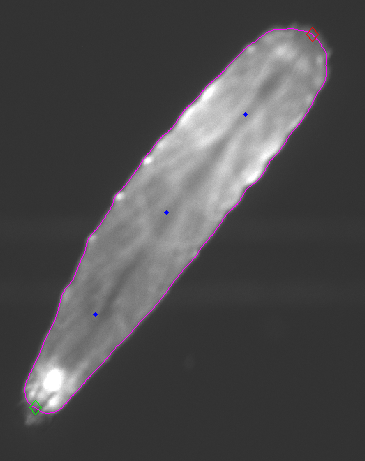
\includegraphics[height=5cm]{larva.png}}
 \parbox{5cm}{\input{length.TpX}\\
    \input{speed.TpX}}
\end{center}
%
%
\end{frame}


%-------------Slide--------------------------------------------------------

\begin{frame}{Intensity profile}
%
%
\begin{center}
 \input{intensity.TpX}
\end{center}
%
%
\end{frame}


%-------------Slide--------------------------------------------------------

\begin{frame}{Period and wavelength from intensity profile}
%
 %
 \begin{center}
 \input{Ixt.TpX}
 \end{center}
 %
%
\end{frame}


%-------------Slide--------------------------------------------------------

\begin{frame}{Fourier transform}
%
 %
 \begin{center}
  \input{Ikw.TpX}
 \end{center}
 %
%
\end{frame}


%-------------Slide--------------------------------------------------------

\begin{frame}{Width of pulse (preliminary)}
%
 %
 \begin{center}
   \input{dIpr.TpX}
   \input{width.TpX}
 \end{center}
 %
%
\end{frame}





% Press Ctrl-D to insert a new slide

%-----End----------------------------------------------------------------

\end{document}
